% !TeX encoding = UTF-8
% !TeX spellcheck = pl_PL

% $Id:$

%Author: Wojciech Domski
%Szablon do ząłożeń projektowych, raportu i dokumentacji z sterowników robotów
%Wersja v.1.0.0
%


%% Konfiguracja:
\newcommand{\kurs}{Sterowniki robot\'{o}w}
\newcommand{\formakursu}{Projekt}

%odkomentuj właściwy typ projektu
\newcommand{\doctype}{Etap II}
%\newcommand{\doctype}{Raport}
%\newcommand{\doctype}{Dokumentacja}

%wpisz nazwę projektu
\newcommand{\projectname}{Miecz \'{S}wietlny}

%wpisz akronim projektu
\newcommand{\acronim}{Mi\'{S}}

%zmaiast X wpisz numer grupy projektowej
\newcommand{\nrgrupy}{4}
%wpisz Imię i nazwisko oraz numer albumu
\newcommand{\osobaA}{Patryk \textsc{Knapik}, 226302}
%w przypadku projektu jednoosobowego usuń zawartość nowej komendy
\newcommand{\osobaB}{Wojciech \textsc{Kosicki}, 234506}

%wpisz termin w formie, jak poniżej dzień, parzystość, godzina
\newcommand{\termin}{wtTP11}

%wpisz imię i nazwisko prowadzącego
\newcommand{\prowadzacy}{mgr in\.{z}. Wojciech \textsc{Domski}}

\documentclass[10pt, a4paper]{article}
% W nawiasie klamrowym podana jest klasa dokumentu. Standardowe klasy artykułu
% to: article, amsart, scrartcl, artikel1, artikel2, artikel3.
% W nawiasie prostokątnym deklarowane są opcje dokumentu. Zamiast 10pt
% można podać 11pt lub 12pt. Dokument w dwóch kolumnach uzyskuje się po
% wpisaniu opcji twocolumn, 

%Preambuła dokumentu

% linki w spisie tresci, bibliografi
\usepackage[bookmarks=true,bookmarksnumbered=false,unicode=true,pdftex=true, colorlinks,filecolor=black,linkcolor=black,urlcolor=black,citecolor=black]{hyperref}

%ustawienie rozmiaru papieru
\usepackage[a4paper, left=2.5cm, right=2.5cm, top=2.5cm, bottom=2.5cm, headsep=1.2cm]{geometry}

%rozmaite ustawienia pozwalające okreslić język

%NALEŻY wybrać jeden z pakietów
%\usepackage{polski} %przydatne podczas składania dokumentów w j. polskim
\usepackage[polish]{babel}  % pakiet lokalizujący dokument w języku polskim
%\usepackage[british]{babel}

\usepackage{indentfirst}	% polski styl pisania (np. rozpoczecie pierwszego akapitu
% pod nazwa rozdzialu od wciecia)
%\usepackage[OT4]{fontenc}
\usepackage[utf8]{inputenc} % w miejsce utf8 można wpisać latin2 bądź cp1250,
% w zależności od tego w jaki sposób kodowane są 
% polskie znaki diakrytyczne przy wprowadzaniu 
% z klawiatury.
%kodowanie znaków, zależne od systemu
\usepackage[T1]{fontenc} %poprawne składanie polskich czcionek

%OPEROWANIE NA OBRAZACH
\usepackage{graphicx}       % pakiet graficzny, umożliwiający m.in.
% import grafik w formacie eps
%\usepackage{epstopdf}		% pozwala na importowanie grafik w formacie eps
% przy użyciu pdflatex
\usepackage[update,prepend]{epstopdf}
\usepackage{rotating}       % pakiet umożliwiający obracanie rysunków
\usepackage{subfigure}      % pakiet umożliwiający tworzenie podrysunków
\usepackage{epic}           % pakiet umożliwiający rysowanie w środowisku latex
\usepackage{psfrag}         % pakiet umożliwiający podmianę łańcuchów znaków 
% w plikach eps
%\usepackage{curves}         % pakiet do wykreslania krzywych

%pakiety dodające dużo dodatkowych poleceń matematycznych
\usepackage{amsfonts}       % pakiet z rozmaitymi czcionkami matematycznymi
%\usepackage{amssymb}        % pakiet z rozmaitymi symbolami matematycznymi
\usepackage{amsmath}        % pakiet z rozmaitymi środowiskami matematycznymi

\usepackage{fp}             % pakiet z funkcjami operujacymi 
% na liczbach zmiennoprzecinkowych
\usepackage{calc}           % pakiet umożliwiający operacje arytmetyczne
% na tzw. licznikach (liczbach całkowitych)
\usepackage{leftidx}		% indeksy górne i dolne po lewej stronie

%definicje matematyczne
\providecommand{\abs}[1]{\lvert#1\rvert}
\providecommand{\norm}[1]{\lVert#1\rVert}

%pakiety wspomagające i poprawiające składanie tabel
\usepackage{supertabular}
\usepackage{array}
\usepackage{tabularx}
\usepackage{hhline}
\usepackage{longtable}		% wsparcie dla dlugich tabel
\usepackage{multicol}		% podzial strony na wiele kolumn

%pakiet do BibTex
\usepackage{cite}

\usepackage{url} %pakiet pozawalający na dodawanie adresów url w bibliografi

%pakiet wypisujący na marginesie etykiety równań i rysunków zdefiniowanych przez \label{}, chcąc wygenerować finalną wersję dokumentu wystarczy usunąć poniższą linię
%\usepackage{showlabels}

\usepackage{float}			% lepsza obsluga mechanizmow obiektow plywajacych
% wymuszenie wstawienia np. tabeli, obrazka w danym miejscu przez [H]

\usepackage{listings}       % pakiet dedykowany zrodlom programow
\usepackage{color}


\definecolor{dkgreen}{rgb}{0,0.6,0}
\definecolor{gray}{rgb}{0.5,0.5,0.5}
\definecolor{mauve}{rgb}{0.58,0,0.82}

\lstset{ %
	language=Matlab,                % the language of the code
	basicstyle=\scriptsize,           % the size of the fonts that are used for the code
	numbers=left,                   % where to put the line-numbers
	numberstyle=\tiny\color{gray},  % the style that is used for the line-numbers
	stepnumber=1,                   % the step between two line-numbers. If it's 1, each line 
	% will be numbered
	numbersep=5pt,                  % how far the line-numbers are from the code
	backgroundcolor=\color{white},      % choose the background color. You must add \usepackage{color}
	showspaces=false,               % show spaces adding particular underscores
	showstringspaces=false,         % underline spaces within strings
	showtabs=false,                 % show tabs within strings adding particular underscores
	%frame=single,                   % adds a frame around the code
	rulecolor=\color{black},        % if not set, the frame-color may be changed on line-breaks within not-black text (e.g. comments (green here))
	tabsize=2,                      % sets default tabsize to 2 spaces
	captionpos=b,                   % sets the caption-position to bottom
	breaklines=true,                % sets automatic line breaking
	breakatwhitespace=false,        % sets if automatic breaks should only happen at whitespace
	%title=\lstname,                   % show the filename of files included with \lstinputlisting;
	% also try caption instead of title
	keywordstyle=\color{blue},          % keyword style
	commentstyle=\color{dkgreen},       % comment style
	stringstyle=\color{mauve},         % string literal style
	escapeinside={\%*}{*)},            % if you want to add LaTeX within your code
	morekeywords={*,...},              % if you want to add more keywords to the set
	deletekeywords={...}              % if you want to delete keywords from the given language
}

%polish signs in lst code
\lstset{literate=%
	{ą}{{\k{a}}}1
	{ć}{{\'c}}1
	{ę}{{\k{e}}}1
	{ł}{{\l}}1
	{ń}{{\'n}}1
	{ó}{{\'o}}1
	{ś}{{\'s}}1
	{ż}{{\.z}}1
	{ź}{{\'z}}1
	{Ą}{{\k{A}}}1
	{Ć}{{\'C}}1
	{Ę}{{\k{E}}}1
	{Ł}{{\L}}1
	{Ń}{{\'N}}1
	{Ó}{{\'O}}1
	{Ś}{{\'S}}1
	{Ż}{{\.Z}}1
	{Ź}{{\'Z}}1
}

\usepackage{verbatim}       % pakiet dedykowany rozmaitym wydrukom tekstowym
\usepackage{ifthen}         % pakiet umożliwiający tworzenie prostych programów
% (m.in. zawiera instrukcje powtórzeniowe 
% i warunkowe)
\usepackage{upquote}		%normal quotations marks ' and `

% deklaracje wymagane przez pakiet theorem automatycznie ladowany w przypadku
% klasy dokumentu article
%
\newtheorem{Dn}{Definicja}[section]     % deklaracja srodowiska definicja
\newtheorem{La}[Dn]{Lemat}                % deklaracja srodowiska lemat
\newtheorem{Tm}[Dn]{Twierdzenie}          % deklaracja srodowiska twierdzenie
\newtheorem{Rk}[Dn]{Spostrze{\.z}enie}  % deklaracja srodowiska spostrzezenie
\newtheorem{Am}[Dn]{Algorytm}           % deklaracja srodowiska algorytm
\newtheorem{As}[Dn]{Za{\l}o{\.z}enie}   % deklaracja srodowiska zalozenie
\newtheorem{Pn}[Dn]{Propozycja}           % deklaracja srodowiska propozycja
\newtheorem{Py}[Dn]{W{\l}asno{\'s}{\'c}}  % deklaracja srodowiska wlasnosc
\newtheorem{Cy}[Dn]{Wniosek}              % deklaracja srodowiska wniosek
\newtheorem{Ee}[Dn]{Przyk{\l}ad}        % deklaracja srodowiska przyklad
\newtheorem{Ex}{{\'C}wiczenie}          % deklaracja srodowiska cwiczenie

%helps to specify width of a column in table
%\begin{tabular}{|C{1cm}|c|c|c|c|c|c|c|c|c|c|}
%first column will have widht of 1cm
\newcolumntype{L}[1]{>{\raggedright\let\newline\\\arraybackslash\hspace{0pt}}m{#1}}
\newcolumntype{C}[1]{>{\centering\let\newline\\\arraybackslash\hspace{0pt}}m{#1}}
\newcolumntype{R}[1]{>{\raggedleft\let\newline\\\arraybackslash\hspace{0pt}}m{#1}}

\sloppy			%zawija bardzo długie linie

%\pagenumbering{gobble}% Remove page numbers (and reset to 1)

	
\begin{document}

\def\tablename{Tabela}	%zmienienie nazwy tabel z Tablica na Tabela

\begin{titlepage}
	\begin{center}
		\textsc{\LARGE \formakursu}\\[1cm]		
		\textsc{\Large \kurs}\\[0.5cm]		
		\rule{\textwidth}{0.08cm}\\[0.4cm]
		{\huge \bfseries \doctype}\\[1cm]
		{\huge \bfseries \projectname}\\[0.5cm]
		{\huge \bfseries \acronim}\\[0.4cm]
		\rule{\textwidth}{0.08cm}\\[1cm]
		
		\begin{flushright} \large
		\emph{Skład grupy (\nrgrupy):}\\
		\osobaA\\
		\osobaB\\[0.4cm]
		
		\emph{Termin: }\termin\\[0.4cm]

		\emph{Prowadzący:} \\
		\prowadzacy \\
		
		\end{flushright}
		
		\vfill
		
		{\large \today}
	\end{center}	
\end{titlepage}

\newpage
\tableofcontents
\newpage

\section{Wstęp}
\label{sec:Wstęp}
Celem projektu jest skonstruowanie miecza świetlnego, który będzie wydawał charakterystyczne dźwięki w zależności od poruszania nim przez użytkownika. 
Niniejszy raport opisuje jakie aspekty projektu udało się z powodzeniem zrealizować do dnia 15 maja 2018 roku. Opisuje także ogólny przebieg prac oraz podjęte decyzje przy rozwiązywaniu problemów. 

\section{Wygenerowanie projektu bazowego w CubeMX}
Pierwszym zadaniem było dobranie odpowiednich peryferiów wykorzystywanych w projekcie i skonfigurowanie ich w środowisku CubeMX. Wygenerowany kod był podstawą do rozpoczęcia pracy nad projektem. 
\begin{enumerate}
		\item Aktywowane PINy
	\begin{figure}[H]
	\centering
	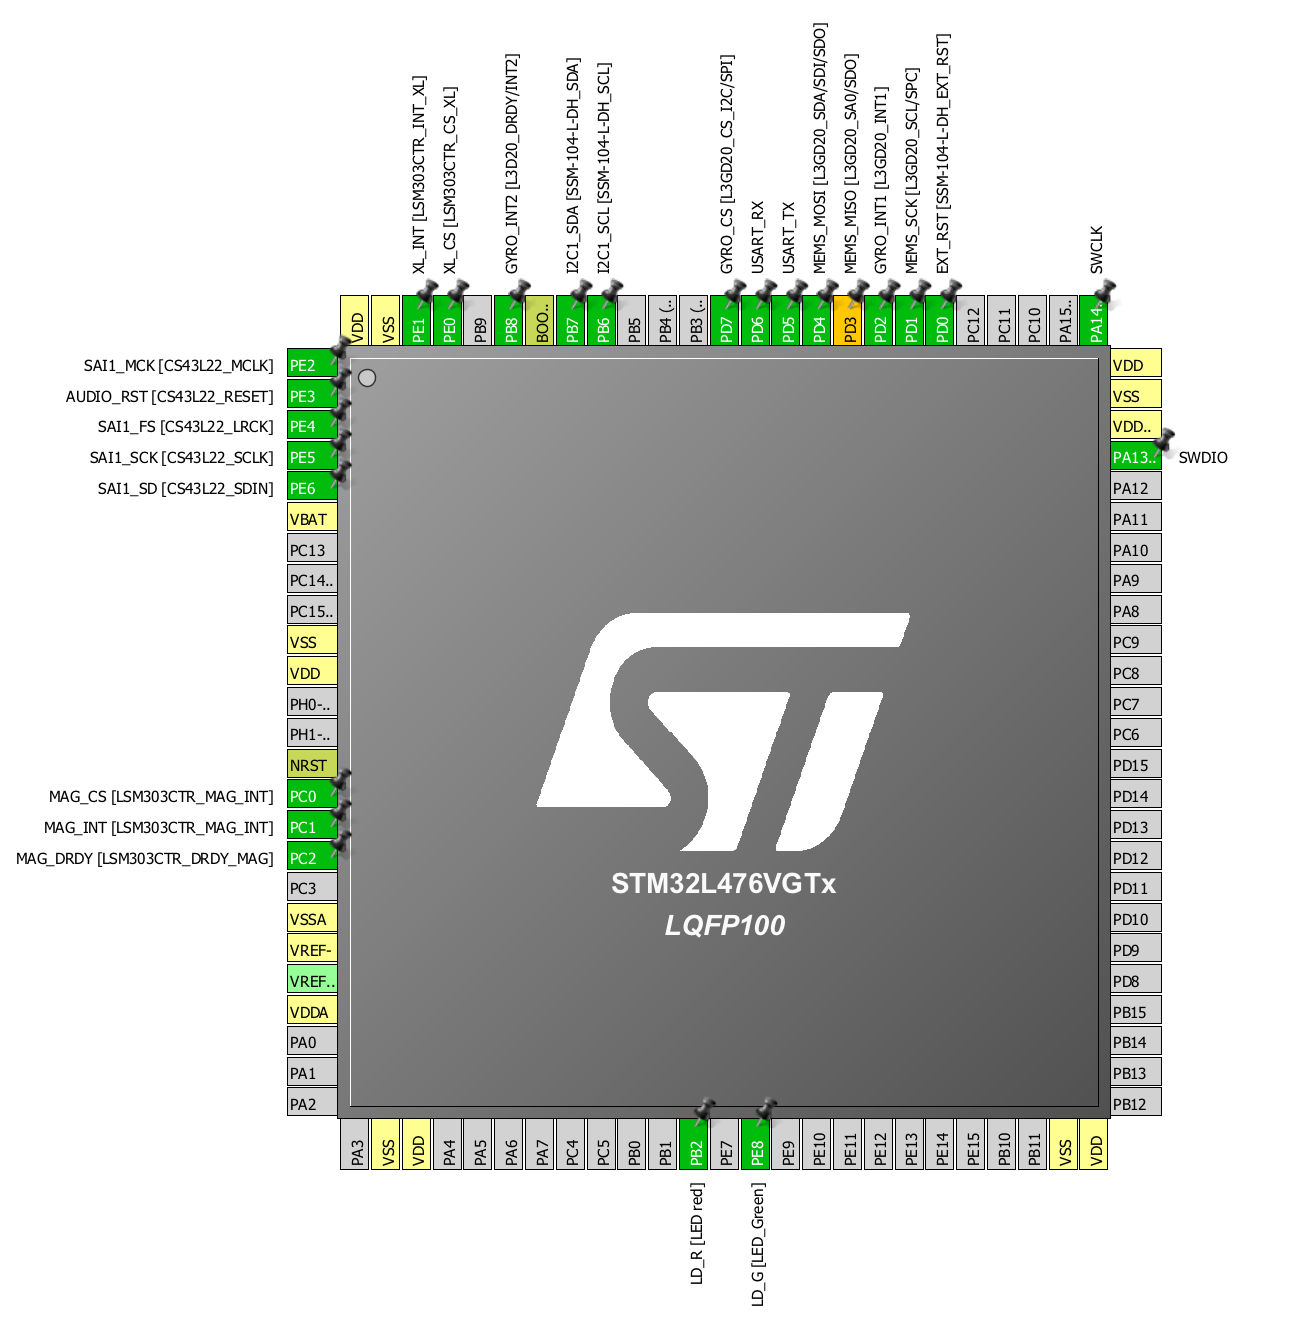
\includegraphics[width=\linewidth]{conf1.png}
	\end{figure}
	\newpage
			\item Konfiguracja zegara
	\begin{figure}[H]
	\centering
	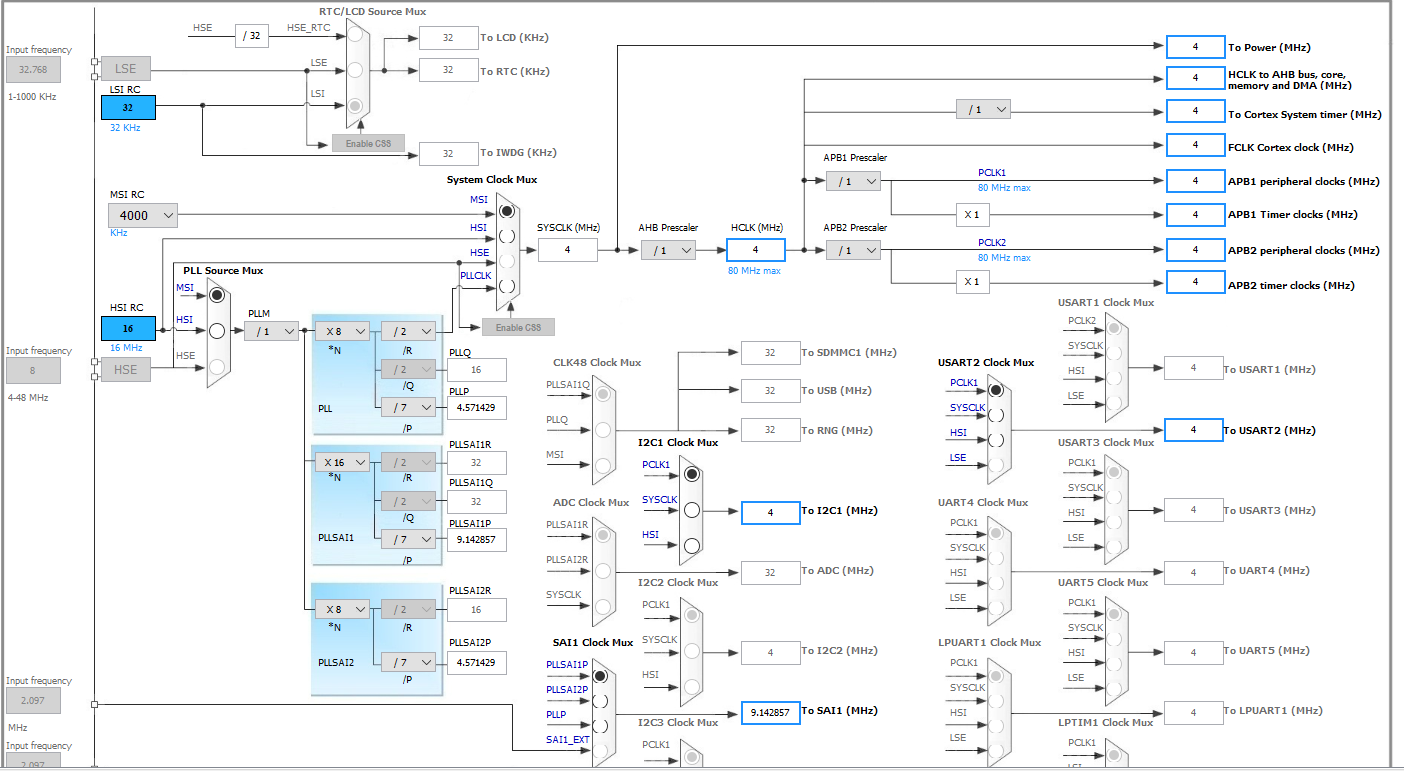
\includegraphics[width=\linewidth]{conf2.png}
	\end{figure}
				\item Okno Middlewares
	\begin{figure}[H]
	\centering
	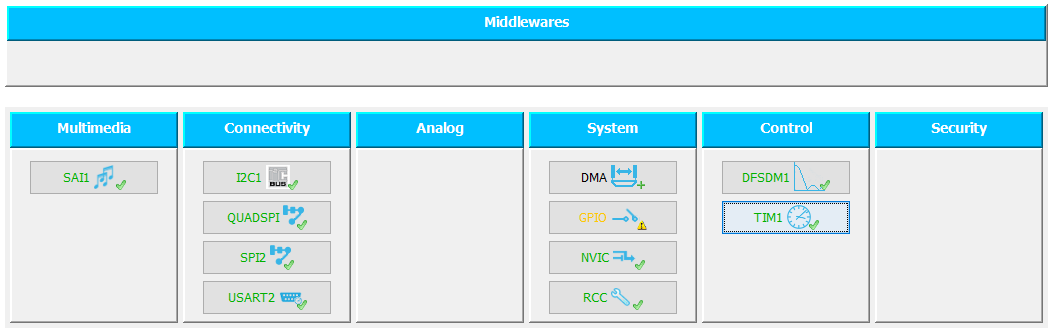
\includegraphics[width=\linewidth]{conf9.png}
	\end{figure}
	\newpage
					\item Ustawienia parametrów
	\begin{figure}[H]
	\centering
	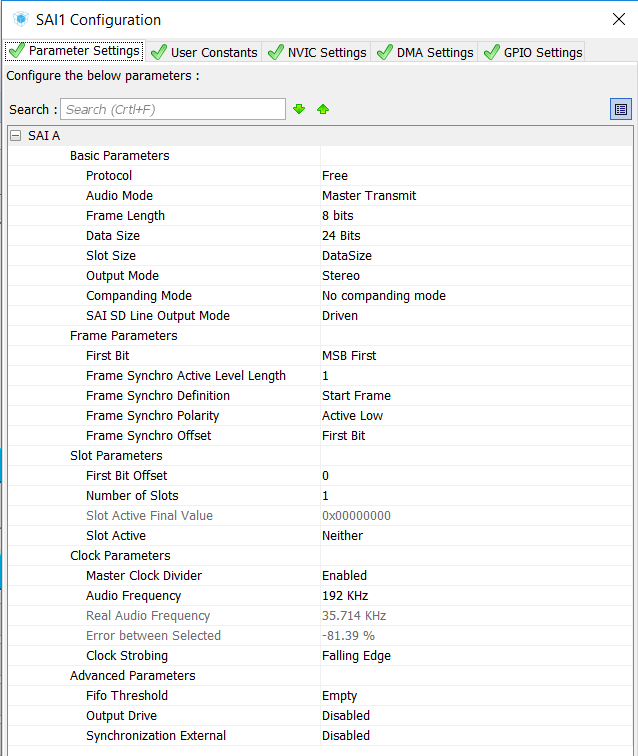
\includegraphics[width=\linewidth]{conf3.png}
	\end{figure}
		\begin{figure}[H]
	\centering
	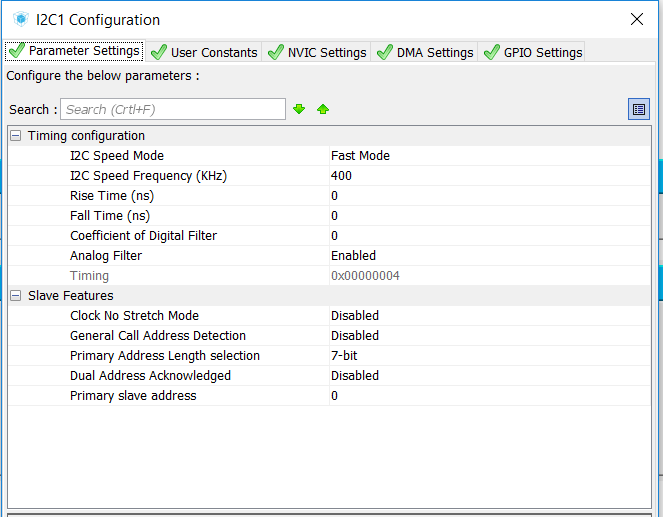
\includegraphics[width=\linewidth]{conf4.png}
	\end{figure}
		\begin{figure}[H]
	\centering
	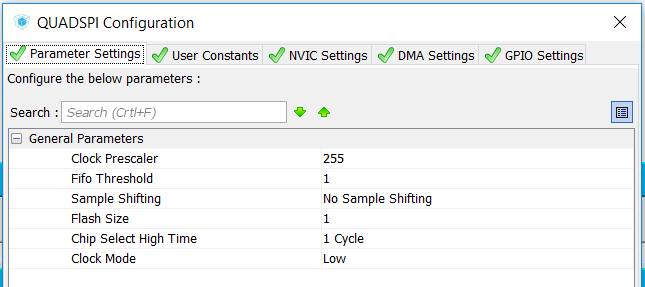
\includegraphics[width=\linewidth]{conf5.png}
	\end{figure}
		\begin{figure}[H]
	\centering
	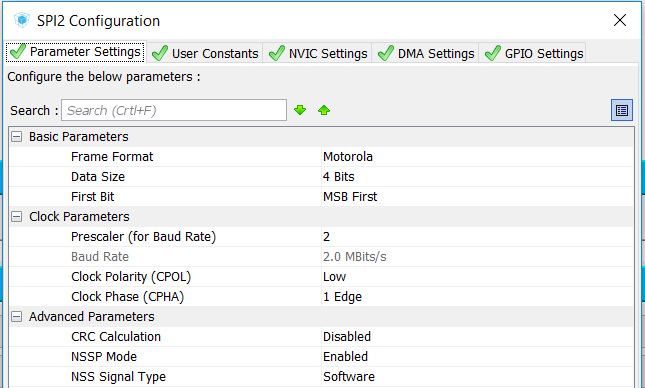
\includegraphics[width=\linewidth]{conf6.png}
	\end{figure}
		\begin{figure}[H]
	\centering
	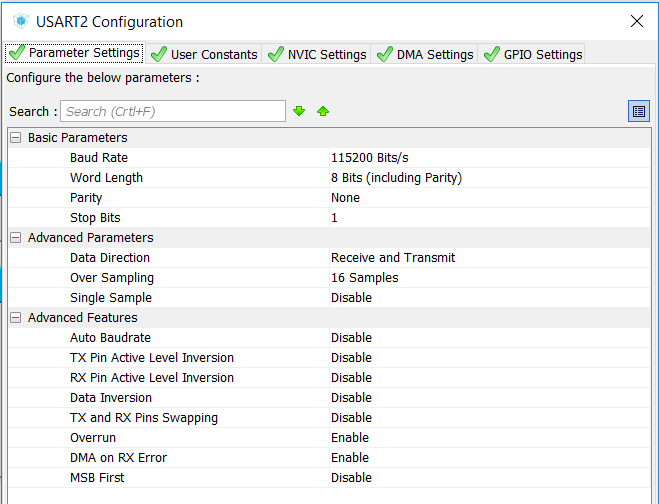
\includegraphics[width=\linewidth]{conf7.png}
	\end{figure}
		\begin{figure}[H]
	\centering
	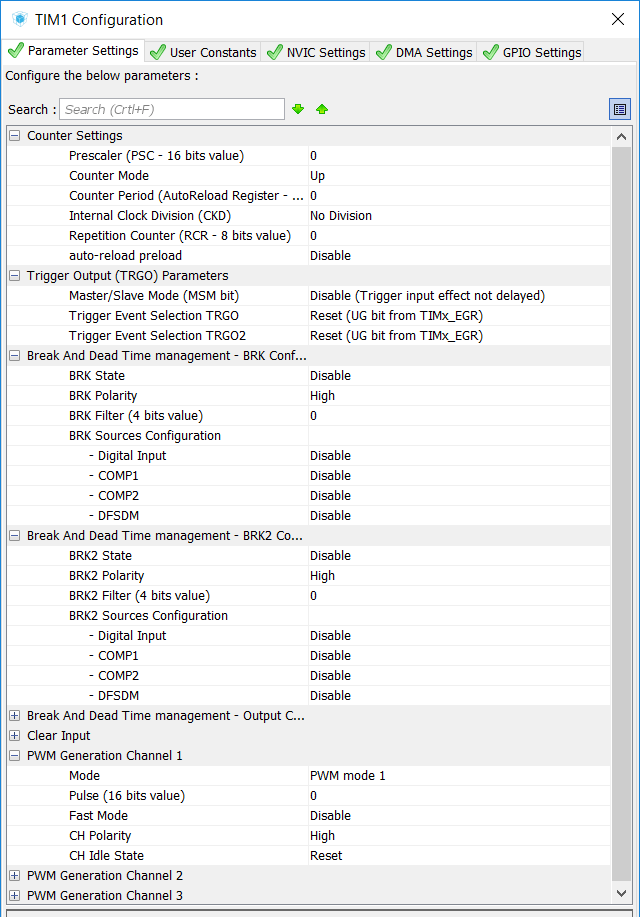
\includegraphics[width=\linewidth]{conf8.png}
	\end{figure}
\end{enumerate}
	\section{Implementacja obsługi DAC}
Płytka STM32L476G-DISCO wyposażona jest w DAC stereo CS43L22 firmy Cirrus Logic. Do zaprogramowania tego peryferium została wykorzystana biblioteka BSP dostarczona przez firmę ST. Urządzenie to konfigurowane jest przez interfejs I$^2$C, a sygnał audio wysyłany jest przez interfejs SAI. Dane audio są kopiowane z pamięci mikrokontrolera na interfejs SAI z wykorzystaniem układu DMA, pozwala to odciążyć rdzeń mikrokontrolera, a także zapewnić płynność dźwięku. Na tym etapie mikrokontroler generuje przebieg sinusoidalny o konfigurowalnej częstotliwości sygnału, a także o zadanej częstotliwości próbkowania, która nie musi być wysoka z uwagi na to, że wysoka dokładność odwzorowania dźwięku nie jest konieczna, w naszym projekcie częstotliwość próbkowania została ustawiona na 16kHz. Z uwagi na to, że rdzeń generuje dźwięk wolniej niż ten jest odtwarzany konieczne jest zastosowanie osobnego buforu do generowania dźwięku i osobnego do jego odtwarzania, po zakończeniu generowania dźwięku w danym buforze, oraz po zakończeniu odtwarzania próbki wskaźniki na bufory zostana zamienione, dzięki temu procesor będzie mógł generować dźwięk podczas gdy inny dźwięk ( o innej częstotliwości) jest odtwarzany bez przeszkód. Obecnie trwają prace nad stworzeniem formuły która pozwoli syntezować dźwięk miecza świetlnego, gdy prace te zostaną zakończone, formuła zostanie przeniesiona do osobnej funkcji która będzie generować dźwięk na bazie odczytu z akcelerometru do zadanego bufora. Budowa sygnału audio jest bardzo prosta, po ustaleniu częstotliwości próbkowania należy wygenerować tablice amplitud które są typu \textit{uint16\_t} czyli liczby z przedziału od 0 do 65535, biorąc pod uwagę, że jedna sekunda dźwięku składa się z wybranej wcześniej ilości próbek. Cyfrowe filtry DFSDM zostały włączone tylko dlatego, że biblioteka audio BSP ich wymaga, ale nie są one wykorzystywane w tym projekcie.
	\section{Implementacja obsługi akcelerometru i żyroskopu}
	Z powodzeniem udało się zaimplementować obsługę akcelerometru poprzez komunikację SPI. Aby odwzorować ruch miecza w bardziej precyzyjny sposób, postanowiono dodać obsługę poprzez komunikację SPI także żyroskopu. Na płytce STM32L476G-DISCO, żyroskop znajduje się na L3GD20, zaś akcelerometr na LSM303C. Wykorzystano dokumentacje w celu zapoznania się odpowiednia konfiguracja i uruchomieniem tych peryferiów. Dużą pomocą były przykładowe funkcje obsługi tych peryferiów w BSP, opublikowanym przez firmę ST. Obsługę tych urządzeń podzielono na dwie warstwy interfejsu. Pierwsza warstwa to napisane biblioteki accel oraz gyros (.c i .h). Druga warstwa zaś to biblioteki lsm i l3g (.c i .h). Zastosowanie dwóch warstw interfejsu może bardzo pomóc w sytuacji gdy trzeba by było przerobić program do działania na innym sterowniku. W takiej sytuacji nie musimy zmieniać całego programu, tylko jedną warstwę interfejsu. 
Postanowiono ustawić wysokie zakresy działania mierników. Dla żyroskopu była to wartość 2000 DPS (stopnie na sekundę), a dla akcelerometru była to wartość 8G (przyśpieszeń ziemskich). Skalibrowano takie ustawienia by nie dochodziło do saturacji odczytów peryferiów. Inaczej, żeby algorytm proporcjonalnie generował dźwięk ruchu miecza w przestrzeni, nawet przy zamaszystych i szybkich ruchach. 
W projekcie zaimplementowano także biblioteki akcelstruct.h oraz gryostruct.h. Zawierają one struktury do inicjalizacji i konfiguracji tych peryferiów. Ostatnią istotną biblioteką napisaną na potrzebę projektu to komun.h/komun.c. Odpowiedzialna jest ona za skonfigurowanie i przeprowadzenie komunikacji przez kanał SPI2. Biblioteka obsługuje inicjalizację i komunikację z zarówno akcelerometrem jak i żyroskopem. 
W celach testowych, odczyty peryferiów były przesyłane przez komunikację UART na komputer, w różnych odstępach czasu. Wyniki testów zakończyły się powodzeniem. Następnym krokiem będzie dostosowanie wyjściowych zmiennych do potrzeb algorytmu generującego dźwięk w głównej pętli programu. 
Idea powiązań klas została przedstawiona na końcu dokumentu:
	\begin{figure}[b]
	\centering
	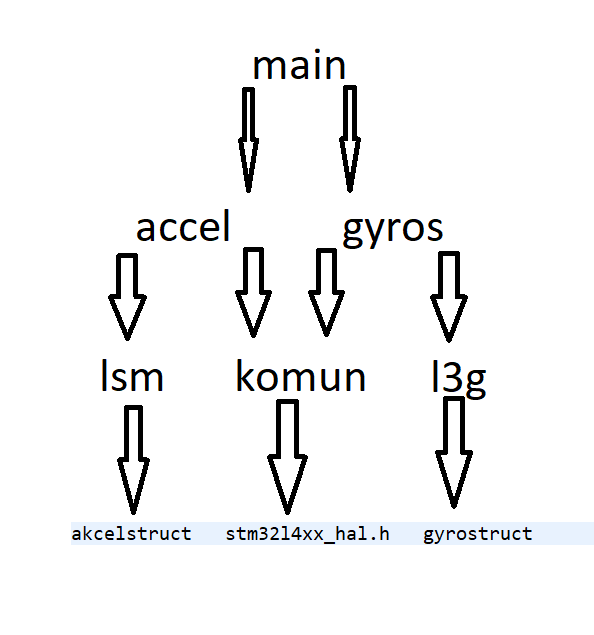
\includegraphics[width=\linewidth]{bilio.png}
	\end{figure}

\section{Projekt miecza świetlnego}	
Do miecza jest wykorzystana zaprojektowana konstrukcja z plexi. W szerszej rękojeści znajduje się sterownik STM32. Oświetlenie miecza bazuje na trzech diodach RGB zamontowanych na początku miecza, w środku i na czubku. Są one sterowane przez sygnał PWM. 
	

\newpage
\addcontentsline{toc}{section}{Bibilografia}
\bibliography{bibliografia}
\bibliographystyle{plain}


\end{document}







































